\subsection{Durham} \label{sec:durham}
Jiang showed that PR scores are significantly correlated to human movement in four areas of London \cite{doi:10.1080/13658810802022822}, and we will use this methodology as a basis for our analysis of vehicle movement in Durham. 
\subsubsection{Methodology}
In order to represent the road network in Durham, we first produce an axial map and then are able to form a connectivity graph. The axial map is produced by taking a map of Durham, Figure \ref{fig:durham map}, and representing the intersections of the roads by a 'The axial map is constructed by taking an accurate map and drawing a set of intersecting lines through all the spaces of the urban grid so that the grid is covered and all rings of circulation are completed.' \cite{Axialmap40:online}, thus forming the axial map in Figure \ref{fig:durham axial}. This axial map can now be represented as a directed hypergraph, Figure \ref{fig:durham graph}. 

\begin{figure}[h]
\centering
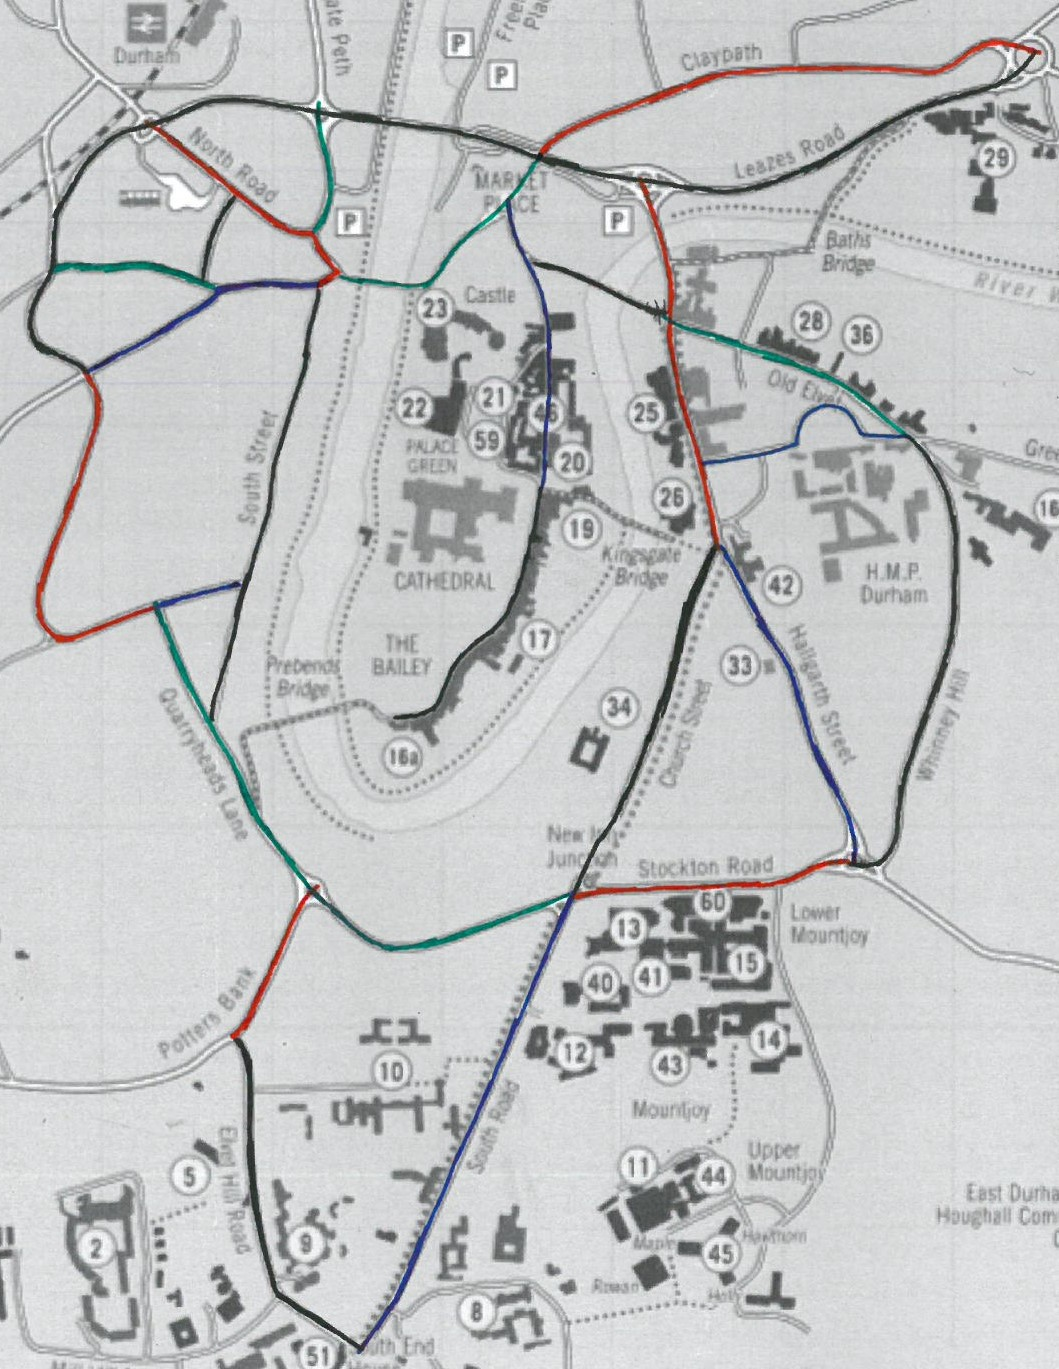
\includegraphics[width=\linewidth]{durham_with_colour.jpg}
\caption{Durham road network, adapted from \cite{undergraduate}}
\label{fig:durham map}
\end{figure}

\begin{figure}[h]
\centering
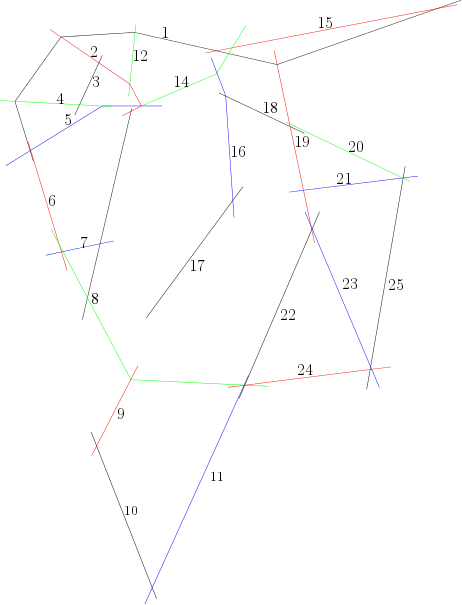
\includegraphics[width=10cm]{axial_colour_label.png}
\caption{Durham road network represented by an axial graph}
\label{fig:durham axial}
\end{figure}

\begin{figure}[h]
\centering
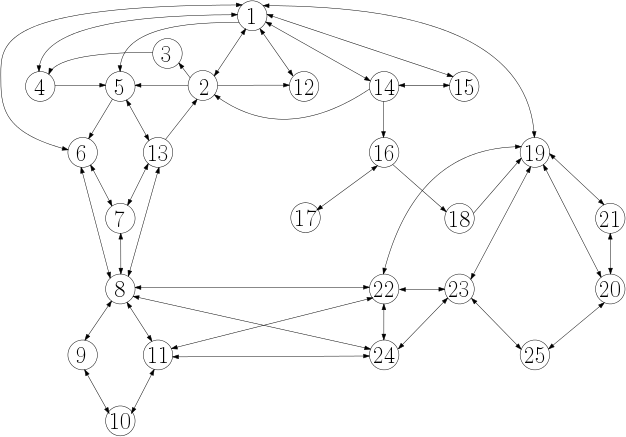
\includegraphics[width=10cm]{ipe_durham.png}
\caption{Durham road network represented by a hypergraph}
\label{fig:durham graph}
\end{figure}
\FloatBarrier


\subsubsection{Results and Analysis} \label{sec:results}

\begin{table}[h] \caption{Comparison of PageRankings produced by standard algorithm and the WPR algorithm on Durham}
 \centering
 \begin{tabular} {r l| c c} 
 \multicolumn{2}{c|}{Node}& PR & WPR \\ [0.5ex] 
 \hline
 1&A390&1&1\\
 2&North Rd&8&8\\
 3&Neville St&19&22\\
 4&Allergate&22&19\\
 5&Crossgate&24&24\\
 6&Margery Ln&6&11\\
 7&Grove St&23&23\\
 8&Quarryheads Ln&11&6\\
 9&Potters Bank&13&2\\
 10&Elvet Hill Rd&7&17\\
 11&South Rd&5&18\\
 12&Milburngate&20&25\\
 13&South St&25&13\\
 14&Silver St&2&14\\
 15&Claypath&9&4\\
 16&Saddler St&10&7\\
 17&Bailey&4&5\\
 18&Elvet Bridge&16&20\\
 19&New Elvet&14&5\\
 20&Old Elvet&12&9\\
 21&Court Ln&15&12\\
 22&Church St&21&10\\
 23&Stockton Rd&17&21\\
 24&Hallgarth St&18&16\\
 25&Whinney Hill&3&3\\
 
 \end{tabular}
 \label{Table:Durham comparison}
\end{table}
\FloatBarrier

\subsubsection{Conclusion} \label{sec:Durham conc}